\chapter{The Training, Validation, and Testing Process}

Suppose a friend gets a copy of the answer key before a math test and memorizes it: question 1 is 42,
question 2 is $-3$, and so on. They score 100\%. Do they know any math? You cannot tell from that test.
You would have to give them new questions.

Machine learning has exactly this problem. A flexible model can memorize the examples it learned from, so
its score on those examples says little about how it will do on new ones. This chapter shows how to grade
a model honestly.

\section{Memorizing Is Not Learning}\index{overfitting}
Imagine you had measured only 12 penguins, and you want to predict body mass from flipper length. You could
fit a straight line through the 12 points. Or a curve: a polynomial of degree 3, or degree 8. A higher
degree means a more flexible curve, which can pass closer to every point. (The \verb|np.polyfit| function
finds the best polynomial of a given degree; the Least Squares chapter shows how.)

To judge the curves fairly, we also look at 50 \emph{other} penguins that the curves never saw.
Figure~\ref{fig:overfit-fits} shows what happens.

\begin{figure}[H]
\centering
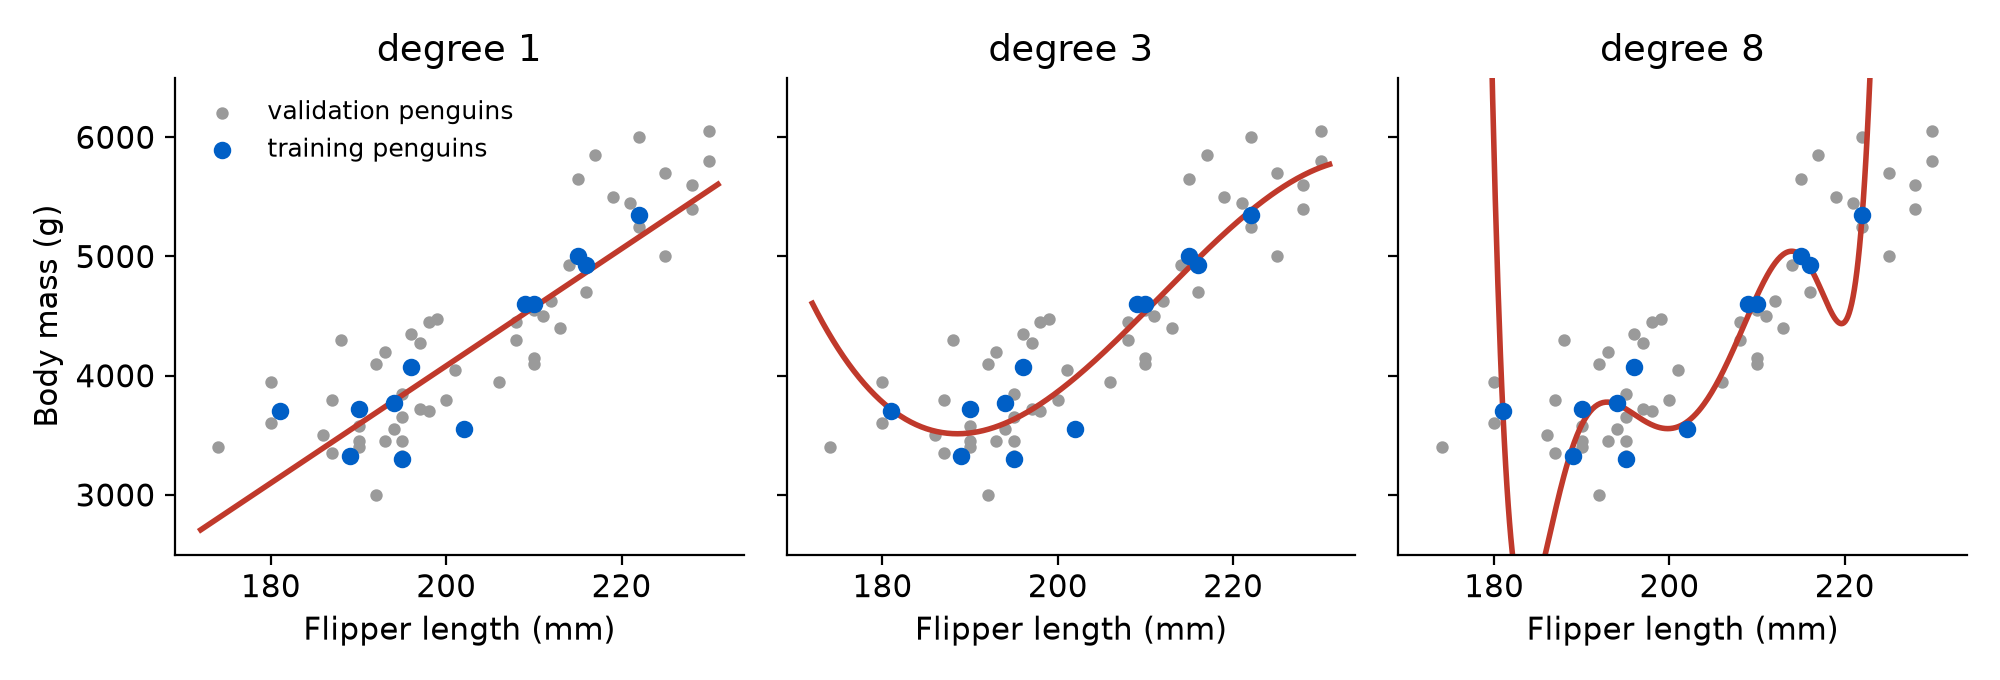
\includegraphics[width=\textwidth]{overfit_fits.png}
\caption{Curves fit to 12 training penguins (blue), judged on 50 validation penguins (gray). The degree-8
curve passes near every training penguin and is wildly wrong almost everywhere else.}
\label{fig:overfit-fits}
\end{figure}

The degree-8 curve wiggles through the training penguins, so its error on them is small. Between and beyond
them, it shoots off to absurd masses. It has memorized the 12 penguins instead of learning the pattern. This
is called \newterm{overfitting}. The opposite problem, a model too simple to capture the pattern, is called
\newterm{underfitting}\index{underfitting}.

Here is the experiment in code. Put \filename{penguins.csv} and \filename{penguins.py} in a folder and create
\filename{overfit.py}:

\begin{minted}{python}
import numpy as np
from penguins import load_penguins

data = load_penguins()
x = data["flipper_length_mm"]
y = data["body_mass_g"]

rng = np.random.default_rng(seed=4)
order = rng.permutation(len(x))
train, val = order[:12], order[12:62]     # only 12 penguins to learn from

# Rescale x so that high powers of it stay reasonable
mean, sd = x[train].mean(), x[train].std()
z = (x - mean) / sd

def rmse(actual, predicted):
    return np.sqrt(np.mean((actual - predicted)**2))

print("degree  train RMSE  val RMSE")
for degree in range(1, 9):
    coefficients = np.polyfit(z[train], y[train], degree)
    train_error = rmse(y[train], np.polyval(coefficients, z[train]))
    val_error = rmse(y[val], np.polyval(coefficients, z[val]))
    print(f"{degree:6d} {train_error:11.0f} {val_error:9.0f}")
\end{minted}

\begin{verbatim}
degree  train RMSE  val RMSE
     1         312       414
     2         239       410
     3         224       386
     4         220       429
     5         219       564
     6         179      6439
     7         179      6562
     8         179     20234
\end{verbatim}

\verb|rng.permutation(n)| shuffles the numbers $0$ to $n - 1$, so \verb|order[:12]| picks 12 random penguins.
Fixing the \verb|seed| makes the shuffle the same every time you run the program.

The two columns tell opposite stories (Figure~\ref{fig:overfit-curve}). The training error falls every time
the curve gets more flexible: more wiggle room always fits the training data better. The validation error
falls a little, then climbs, and finally explodes. \textbf{Only the validation error tells you how the model will
do on penguins it has not seen.}

\begin{figure}[H]
\centering
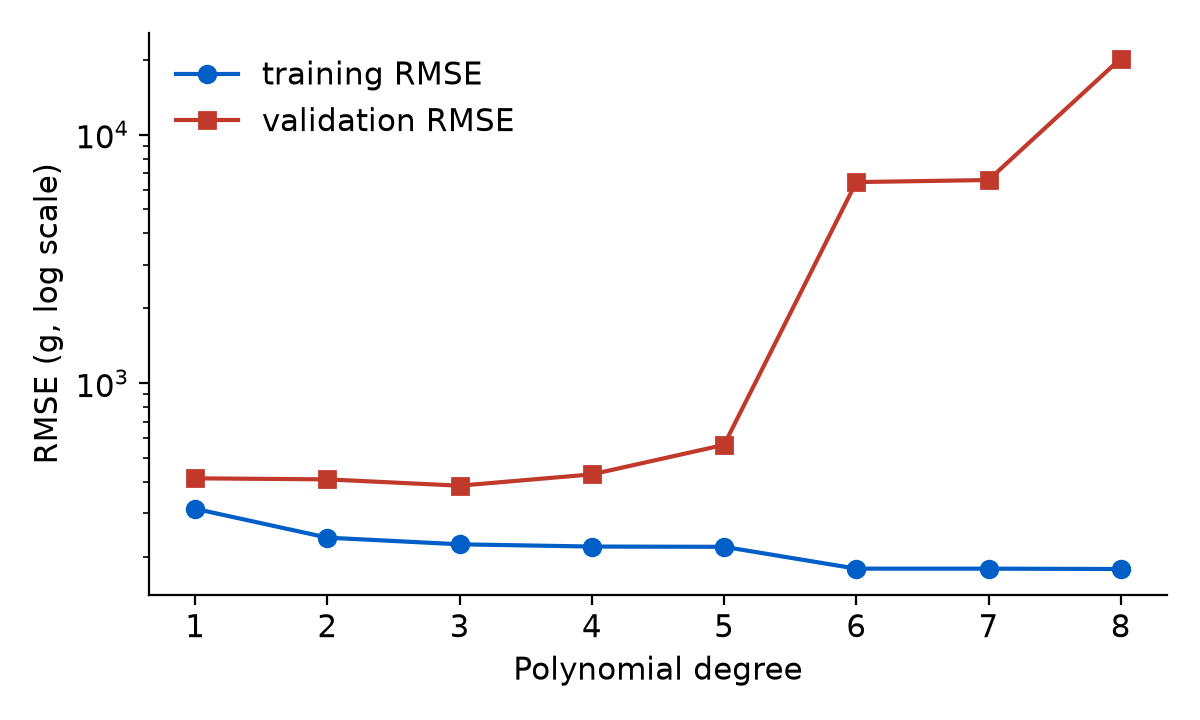
\includegraphics[width=0.7\textwidth]{overfit_curve.png}
\caption{Training error keeps falling as the degree rises. Validation error has a minimum, then rises
sharply. The gap between them is the signature of overfitting.}
\label{fig:overfit-curve}
\end{figure}

\section{Three Sets}\index{training set}\index{validation set}\index{test set}
To grade honestly, split the data into three sets before you do anything else. Think of a math class:
homework is for learning (training), practice tests tell you whether your study strategy is working so you
can adjust it (validation), and the final exam measures what you really know, and it only counts if you have
never seen its questions (testing).

\begin{figure}[H]
\centering
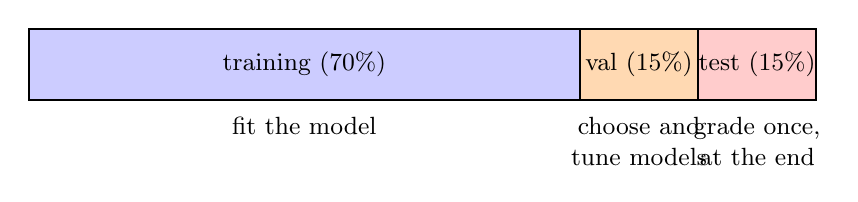
\begin{tikzpicture}[font=\small]
  \fill[blue!20] (0,0) rectangle (7,0.9);
  \fill[orange!30] (7,0) rectangle (8.5,0.9);
  \fill[red!20] (8.5,0) rectangle (10,0.9);
  \draw[thick] (0,0) rectangle (10,0.9) (7,0) -- (7,0.9) (8.5,0) -- (8.5,0.9);
  \node at (3.5,0.45) {training (70\%)};
  \node at (7.75,0.45) {val (15\%)};
  \node at (9.25,0.45) {test (15\%)};
  \node[below, align=center] at (3.5,-0.1) {fit the model};
  \node[below, align=center] at (7.75,-0.1) {choose and\\tune models};
  \node[below, align=center] at (9.25,-0.1) {grade once,\\at the end};
\end{tikzpicture}
\caption{A common way to split the data. Shuffle first.}
\label{fig:three-sets}
\end{figure}

\begin{itemize}
\item The \newterm{training set} is used to fit the model: to find the coefficients of a curve, or the splits
in a decision tree.
\item The \newterm{validation set} is used to compare models and to choose
\newterm{hyperparameters}\index{hyperparameter}: settings that the training does not choose for you, such as
the degree of a polynomial or the number of neighbors $k$ in the $k$-nearest-neighbors method.
\item The \newterm{test set} is used once, at the very end, to estimate how the final model will do on new
data.
\end{itemize}

\textbf{Example}: A data set has 1,000 rows. How many go in each set with a 70/15/15 split?

\textbf{Solution}: 700 training rows, 150 validation rows, and 150 test rows.

Shuffle the rows first, so each set looks like the whole data set. This matters most when the file is sorted:
\filename{penguins.csv} lists all the Adelies first, then the Gentoos, then the Chinstraps, so without shuffling,
the test set would be 50 Chinstraps and nothing else. Here is a shuffled split, \filename{split.py}:

\begin{minted}{python}
import numpy as np
from penguins import load_penguins

data = load_penguins()
n = len(data["species"])

rng = np.random.default_rng(seed=1)    # a fixed seed makes the shuffle repeatable
order = rng.permutation(n)             # the numbers 0 to n-1, shuffled

n_train = int(0.70 * n)
n_val = int(0.15 * n)
train = order[:n_train]
val = order[n_train:n_train + n_val]
test = order[n_train + n_val:]
print("Sizes:", len(train), len(val), len(test))

for name, rows in [("train", train), ("val", val), ("test", test)]:
    kinds, counts = np.unique(data["species"][rows], return_counts=True)
    shares = ", ".join(f"{k} {c / len(rows):.0%}" for k, c in zip(kinds, counts))
    print(f"{name:5s} {shares}")
\end{minted}

\begin{verbatim}
Sizes: 233 49 51
train Adelie 45%, Chinstrap 18%, Gentoo 37%
val   Adelie 39%, Chinstrap 29%, Gentoo 33%
test  Adelie 45%, Chinstrap 24%, Gentoo 31%
\end{verbatim}

\verb|train|, \verb|val|, and \verb|test| are arrays of row numbers. Indexing an array with an array of row
numbers, as in \verb|data["species"][rows]|, picks out just those rows.

Even after shuffling, the small sets wander: Chinstraps are 18\% of the training set but 29\% of the
validation set. For classification, it is often better to shuffle and split each class separately, so every
set keeps the same mix. That is called a \newterm{stratified split}\index{stratified split} (an exercise asks
you to write one).

\section{The Rules}
The three sets only work if they stay separate.
\begin{itemize}
\item \textbf{Never fit anything on the validation or test set.} That includes the coefficients, and also
things like the mean and standard deviation you use to rescale the data. In \filename{overfit.py}, the
rescaling uses \verb|x[train]| only.
\item \textbf{Never choose a model because of its test score.} If you try ten models and keep the one with the
best test score, the test set has become a second validation set, and its score is too optimistic.
\item \textbf{Watch for leaks.} \newterm{Data leakage}\index{data leakage} is any way information from the
validation or test set sneaks into training.
\end{itemize}

Leaks are easy to create by accident:

\begin{center}
\begin{tabular}{>{\raggedright\arraybackslash}p{5.3cm} >{\raggedright\arraybackslash}p{6.2cm}}
\textbf{Leak} & \textbf{Why it is a problem} \\
\hline
Rescaling with the mean of all the data & The test rows helped shape the training data. \\
The same penguin appears twice, once in training and once in testing & The model is graded on a penguin it memorized. \\
Predicting next week's sales with a random split of the dates & The model learns from the future to ``predict'' the past. For data over time, train on earlier dates and test on later ones. \\
A feature that is really the answer, such as ``was flagged as spam'' in a spam filter & The model looks perfect and fails on real data, where that feature does not exist yet. \\
\end{tabular}
\end{center}

\section{Cross-Validation}\index{cross-validation}
With only a few hundred penguins, a 50-penguin validation set is small, and its score depends a lot on which
penguins happened to land in it. \newterm{$k$-fold cross-validation} uses the training data more thoroughly.
Split the training rows into $k$ equal groups, called \newterm{folds}\index{fold}. Train $k$ times, each time
holding out a different fold for validation, and average the $k$ validation scores
(Figure~\ref{fig:kfold}). The test set stays locked away the whole time.

\begin{figure}[H]
\centering
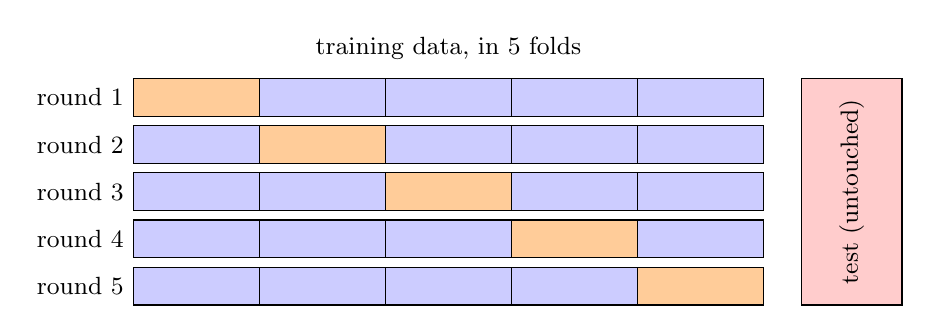
\begin{tikzpicture}[font=\small, x=1.6cm, y=0.6cm]
  \foreach \r in {1,...,5} {
    \foreach \c in {1,...,5} {
      \ifnum\r=\c
        \fill[orange!40] (\c-1,-\r) rectangle (\c,-\r+0.8);
      \else
        \fill[blue!20] (\c-1,-\r) rectangle (\c,-\r+0.8);
      \fi
      \draw (\c-1,-\r) rectangle (\c,-\r+0.8);
    }
    \node[left] at (0,-\r+0.4) {round \r};
  }
  \fill[red!20] (5.3,-5) rectangle (6.1,-0.2);
  \draw (5.3,-5) rectangle (6.1,-0.2);
  \node[rotate=90] at (5.7,-2.6) {test (untouched)};
  \node[above] at (2.5,0) {training data, in 5 folds};
\end{tikzpicture}
\caption{5-fold cross-validation. In each round, the orange fold is the validation set and the blue folds
are for training. Every training row is used for validation exactly once.}
\label{fig:kfold}
\end{figure}

Let us use 5-fold cross-validation, with all the penguins this time, to choose the polynomial degree.
Create \filename{crossval.py}:

\begin{minted}{python}
import numpy as np
from penguins import load_penguins

data = load_penguins()
x = data["flipper_length_mm"]
y = data["body_mass_g"]

rng = np.random.default_rng(seed=1)
order = rng.permutation(len(x))
n_test = 50
test, train = order[:n_test], order[n_test:]   # lock the test set away

mean, sd = x[train].mean(), x[train].std()
z = (x - mean) / sd

def rmse(actual, predicted):
    return np.sqrt(np.mean((actual - predicted)**2))

k = 5
folds = np.array_split(train, k)        # 5 groups of training rows

print("degree  cross-validated RMSE")
scores = {}
for degree in range(1, 6):
    errors = []
    for i in range(k):
        held_out = folds[i]
        fit_rows = np.concatenate([folds[j] for j in range(k) if j != i])
        coefficients = np.polyfit(z[fit_rows], y[fit_rows], degree)
        errors.append(rmse(y[held_out], np.polyval(coefficients, z[held_out])))
    scores[degree] = np.mean(errors)
    print(f"{degree:6d} {scores[degree]:12.1f}")

best = min(scores, key=scores.get)
coefficients = np.polyfit(z[train], y[train], best)
print(f"Chose degree {best}. Test RMSE: {rmse(y[test], np.polyval(coefficients, z[test])):.1f}")
\end{minted}

\begin{verbatim}
degree  cross-validated RMSE
     1        389.6
     2        376.1
     3        371.1
     4        370.6
     5        371.5
Chose degree 4. Test RMSE: 407.2
\end{verbatim}

\verb|np.array_split| cuts an array into nearly equal pieces, and \verb|min(scores, key=scores.get)| finds the
dictionary key with the smallest value.

With 283 penguins to learn from instead of 12, overfitting is much milder: degrees 2 through 5 all score
within about 6 g of each other. The program picks degree 4, but its lead over degree 3 is half a gram, far less
than the variation between folds (about 16 g). When scores are this close, most data scientists choose the
\emph{simplest} model that is about as good as the best one, since simpler models are easier to understand and
less likely to have overfit. One exercise makes this precise.

Notice also that the test RMSE (407 g) is higher than the cross-validated estimate (371 g). That is normal:
choosing the best of several models makes its validation score a little optimistic, which is exactly why the
untouched test set exists.

\begin{Exercise}[label=tvt1, title=Count the rows]
A data set has 2,400 rows, split 70\% training, 15\% validation, and 15\% testing. How many rows are in each
set?
\end{Exercise}
\begin{Answer}[ref=tvt1]
Training: $0.70 \cdot 2400 = 1680$. Validation: $0.15 \cdot 2400 = 360$. Testing: $360$.
\end{Answer}

\begin{Exercise}[label=tvt2, title=Spot the leak]
A student rescales every feature using the mean and standard deviation of all 1,000 rows, and then splits
the data. Explain why this is a problem.
\end{Exercise}
\begin{Answer}[ref=tvt2]
The mean and standard deviation of the validation and test rows were used when rescaling the training rows,
so information from the test set leaked into training. The fix is to compute the rescaling from the training
set only, and then apply it to the other sets.
\end{Answer}

\begin{Exercise}[label=tvt3, title=Which set?]
A researcher tries 10 values of $k$ for a $k$-nearest-neighbors model and picks the one with the best test
score. What is wrong with this?
\end{Exercise}
\begin{Answer}[ref=tvt3]
The choice of $k$ should be made on the validation set (or by cross-validation). Picking it by the test score
means the test set has been used for tuning, so the reported test score is optimistic.
\end{Answer}

\begin{Exercise}[label=tvt4, title=Read the curve]
In Figure~\ref{fig:overfit-curve}, which degrees underfit, and which overfit? Which degree would you choose
using the validation set?
\end{Exercise}
\begin{Answer}[ref=tvt4]
Degree 1 underfits a little: both errors are higher than they need to be. From degree 5 on, the models
overfit: training error keeps dropping while validation error rises, sharply after degree 5. Degree 3 has
the lowest validation error (386 g), so the validation set picks degree 3.
\end{Answer}

\begin{Exercise}[label=tvt5, title=A stratified split]
Change \filename{split.py} so that it shuffles and splits each species separately, putting 70\% of each
species in training, 15\% in validation, and the rest in testing. Check that the three sets now have nearly
the same species mix.
\end{Exercise}
\begin{Answer}[ref=tvt5]
\begin{minted}{python}
species = data["species"]
train, val, test = [], [], []
for kind in np.unique(species):
    rows = rng.permutation(np.flatnonzero(species == kind))
    a, b = int(0.70 * len(rows)), int(0.85 * len(rows))
    train += list(rows[:a])
    val += list(rows[a:b])
    test += list(rows[b:])
\end{minted}
\verb|np.flatnonzero(species == kind)| gives the row numbers of one species. Printing the shares as before gives
\begin{verbatim}
train 232 Adelie 44%, Chinstrap 20%, Gentoo 36%
val 50 Adelie 44%, Chinstrap 20%, Gentoo 36%
test 51 Adelie 43%, Chinstrap 22%, Gentoo 35%
\end{verbatim}
\end{Answer}

\begin{Exercise}[label=tvt6, title={The one-standard-error rule}]
In \filename{crossval.py}, also compute the \emph{standard error} of each degree's five fold scores, which is
their standard deviation divided by $\sqrt{5}$. The \newterm{one-standard-error rule}\index{one-standard-error
rule} says: find the best score, add its standard error, and choose the simplest model whose score is below
that line. Which degree does it choose?
\end{Exercise}
\begin{Answer}[ref=tvt6]
Add \verb|np.std(errors, ddof=1) / np.sqrt(k)| to the printout. The standard errors are all about 15 to 17 g:
\begin{verbatim}
degree  CV RMSE  standard error
     1    389.6   16.6
     2    376.1   16.0
     3    371.1   15.4
     4    370.6   15.3
     5    371.5   15.6
\end{verbatim}
The best score is $370.6$, and $370.6 + 15.3 = 385.9$. The simplest degree under that line is degree 2. (Its
test RMSE is about 412 g, essentially the same as degree 4's 407 g.)
\end{Answer}
